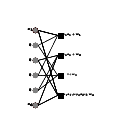
\begin{tikzpicture}
\def\horzgap{0.125in}; %Horizontal gap between nodes/levels
\def \gapVN{0.075in}; %vertical gap between nodes
\def \gapCN{0.1in}; %Horizontal gap between nodes


\def\nodewidth{0.025in};
\def\nodewidthA{0.025in};
\def \edgewidth{0.01in};
\def\ext{0.1in};


\tikzstyle{check} = [rectangle, draw,line width=0.05mm,  inner sep=0mm, fill=black, minimum height=\nodewidthA, minimum width=\nodewidthA]
\tikzstyle{bit} = [circle, draw, line width=0.05mm, inner sep=0mm, fill=red, minimum size=\nodewidthA]
\tikzstyle{bituncover} = [circle, draw=none, line width=0.05mm, inner sep=0mm, fill=gray, minimum size=\nodewidthA]

\tikzstyle{edgesock} = [circle, inner sep=0mm, minimum size=\edgewidth,draw, fill=white]     

             
\onslide<1>{             
\foreach \vn in {1,...,6}{
 \node[bit] (vn\vn) at (0,-\vn*\gapVN) {};
}

\foreach \vn in {2,3,4,5}{
\path (vn\vn) ++(-\nodewidth,0) node()[scale=0.25, inner sep=0mm] {\tiny{0}};
}

\path (vn1) ++(-\nodewidth,0) node()[scale=0.25, inner sep=0mm] {\tiny{$x_{1}$}};
\path (vn6) ++(-\nodewidth,0) node()[scale=0.25, inner sep=0mm] {\tiny{$x_{6}$}};


\foreach \cn in {1,...,4}{
\node[check] (cn\cn) at (\horzgap,-\cn*\gapCN) {};
}

\draw[line width=0.05mm] (vn6.east)--(cn4.west);
\draw[line width=0.05mm] (vn3.east)--(cn4.west);
\draw[line width=0.05mm] (vn1.east)--(cn4.west);

\draw[line width=0.05mm] (vn2.east)--(cn3.west);
\draw[line width=0.05mm] (vn4.east)--(cn3.west);
\draw[line width=0.05mm] (vn5.east)--(cn3.west);

\draw[line width=0.05mm] (vn2.east)--(cn3.west);
\draw[line width=0.05mm] (vn4.east)--(cn3.west);
\draw[line width=0.05mm] (vn5.east)--(cn3.west);

\draw[line width=0.05mm] (vn6.east)--(cn2.west);
\draw[line width=0.05mm] (vn5.east)--(cn2.west);
\draw[line width=0.05mm] (vn3.east)--(cn2.west);

\draw[line width=0.05mm] (vn1.east)--(cn1.west);
\draw[line width=0.05mm] (vn2.east)--(cn1.west);
\draw[line width=0.05mm] (vn4.east)--(cn1.west);

\def\moveX {1.8*\nodewidth};
\def\moveXA {2*\nodewidth};

\path (cn1.east)++(\moveX,0) node ()[scale=0.2] {\tiny{$x_1\mathbf{s}_1+\mathbf{w_{1}}$}};
\path (cn2.east)++(\moveX,0) node ()[scale=0.2] {\tiny{$x_6\mathbf{s}_6+\mathbf{w_{2}}$}};
\path (cn3.east)++(\moveX,0) node ()[scale=0.2] {\tiny{0+$\mathbf{w_{3}}$}};
\path (cn4.east)++(1.75*\moveX,0) node ()[scale=0.2] {\tiny{$x_1\mathbf{s}_1+x_6\mathbf{s}_6+\mathbf{w_{4}}$}};

}

%-----------------------*(&^#@$^&*(^%$^&*(&^--------------------------------------------------------------------
\onslide<2>{
\foreach \vn in {1,3,6}{
 \node[bit] (vn\vn) at (0,-\vn*\gapVN) {};
}

\foreach \vn in {2,4,5}{
 \node[bituncover] (vn\vn) at (0,-\vn*\gapVN) {};
}

\foreach \vn in {2,3,4,5}{
\path (vn\vn) ++(-\nodewidth,0) node()[scale=0.25, inner sep=0mm] {\tiny{0}};
}


\path (vn1) ++(-\nodewidth,0) node()[scale=0.25, inner sep=0mm] {\tiny{$x_{1}$}};
\path (vn6) ++(-\nodewidth,0) node()[scale=0.25, inner sep=0mm] {\tiny{$x_{6}$}};


\foreach \cn in {1,...,4}{
\node[check] (cn\cn) at (\horzgap,-\cn*\gapCN) {};
}

\draw[line width=0.05mm] (vn6.east)--(cn4.west);
\draw[line width=0.05mm] (vn3.east)--(cn4.west);
\draw[line width=0.05mm] (vn1.east)--(cn4.west);

\draw[line width=0.05mm, densely dotted] (vn2.east)--(cn3.west);
\draw[line width=0.05mm, densely dotted] (vn4.east)--(cn3.west);
\draw[line width=0.05mm, densely dotted] (vn5.east)--(cn3.west);

\draw[line width=0.05mm] (vn6.east)--(cn2.west);
\draw[line width=0.05mm] (vn5.east)--(cn2.west);
\draw[line width=0.05mm] (vn3.east)--(cn2.west);

\draw[line width=0.05mm] (vn1.east)--(cn1.west);
\draw[line width=0.05mm] (vn2.east)--(cn1.west);
\draw[line width=0.05mm] (vn4.east)--(cn1.west);

\def\moveX {1.8*\nodewidth};
\def\moveXA {2*\nodewidth};

\path (cn1.east)++(\moveX,0) node ()[scale=0.2] {\tiny{$x_1\mathbf{s}_1+\mathbf{w_{1}}$}};
\path (cn2.east)++(\moveX,0) node ()[scale=0.2] {\tiny{$x_6\mathbf{s}_6+\mathbf{w_{2}}$}};
\path (cn3.east)++(\moveX,0) node ()[scale=0.2] {\tiny{0+$\mathbf{w_{3}}$}};
\path (cn4.east)++(1.75*\moveX,0) node ()[scale=0.2] {\tiny{$x_1\mathbf{s}_1+x_6\mathbf{s}_6+\mathbf{w_{4}}$}};
}
%----------------------------------^%$#@%^&*()_*&^%$#^&*------------------------------------
\onslide<3>{
\foreach \vn in {1,3,6}{
 \node[bit] (vn\vn) at (0,-\vn*\gapVN) {};
}

\foreach \vn in {2,4,5}{
 \node[bituncover] (vn\vn) at (0,-\vn*\gapVN) {};
}

\foreach \vn in {2,3,4,5}{
\path (vn\vn) ++(-\nodewidth,0) node()[scale=0.25, inner sep=0mm] {\tiny{0}};
}


\path (vn1) ++(-\nodewidth,0) node()[scale=0.25, inner sep=0mm] {\tiny{$x_{1}$}};
\path (vn6) ++(-\nodewidth,0) node()[scale=0.25, inner sep=0mm] {\tiny{$x_{6}$}};


\foreach \cn in {1,...,4}{
\node[check] (cn\cn) at (\horzgap,-\cn*\gapCN) {};
}

\draw[line width=0.05mm] (vn6.east)--(cn4.west);
\draw[line width=0.05mm] (vn3.east)--(cn4.west);
\draw[line width=0.05mm] (vn1.east)--(cn4.west);

\draw[line width=0.05mm, densely dotted] (vn2.east)--(cn3.west);
\draw[line width=0.05mm, densely dotted] (vn4.east)--(cn3.west);
\draw[line width=0.05mm, densely dotted] (vn5.east)--(cn3.west);

\draw[line width=0.05mm] (vn6.east)--(cn2.west);
\draw[line width=0.05mm, densely dotted] (vn5.east)--(cn2.west);
\draw[line width=0.05mm] (vn3.east)--(cn2.west);

\draw[line width=0.05mm] (vn1.east)--(cn1.west);
\draw[line width=0.05mm, densely dotted] (vn2.east)--(cn1.west);
\draw[line width=0.05mm, densely dotted] (vn4.east)--(cn1.west);

\def\moveX {1.8*\nodewidth};
\def\moveXA {2*\nodewidth};

\path (cn1.east)++(\moveX,0) node ()[scale=0.2] {\tiny{$x_1\mathbf{s}_1+\mathbf{w_{1}}$}};
\path (cn2.east)++(\moveX,0) node ()[scale=0.2] {\tiny{$x_6\mathbf{s}_6+\mathbf{w_{2}}$}};
\path (cn3.east)++(\moveX,0) node ()[scale=0.2] {\tiny{0+$\mathbf{w_{3}}$}};
\path (cn4.east)++(1.75*\moveX,0) node ()[scale=0.2] {\tiny{$x_1\mathbf{s}_1+x_6\mathbf{s}_6+\mathbf{w_{4}}$}};
}


%----------------------------------^%$#@%^&*()_*&^%$#^&*------------------------------------
\onslide<4>{
\foreach \vn in {1,3,6}{
 \node[bit] (vn\vn) at (0,-\vn*\gapVN) {};
}

\foreach \vn in {2,4,5}{
 \node[bituncover] (vn\vn) at (0,-\vn*\gapVN) {};
}

\foreach \vn in {2,3,4,5}{
\path (vn\vn) ++(-\nodewidth,0) node()[scale=0.25, inner sep=0mm] {\tiny{0}};
}


\path (vn1) ++(-\nodewidth,0) node()[scale=0.25, inner sep=0mm] {\tiny{$x_{1}$}};
\path (vn6) ++(-\nodewidth,0) node()[scale=0.25, inner sep=0mm] {\tiny{$x_{6}$}};


\foreach \cn in {1,...,4}{
\node[check] (cn\cn) at (\horzgap,-\cn*\gapCN) {};
}

\draw[line width=0.05mm] (vn6.east)--(cn4.west);
\draw[line width=0.05mm] (vn3.east)--(cn4.west);
\draw[line width=0.05mm] (vn1.east)--(cn4.west);

\draw[line width=0.05mm] (vn6.east)--(cn2.west);
\draw[line width=0.05mm] (vn3.east)--(cn2.west);

\draw[line width=0.05mm] (vn1.east)--(cn1.west);

\def\moveX {1.8*\nodewidth};
\def\moveXA {2*\nodewidth};

\path (cn1.east)++(\moveX,0) node ()[scale=0.2] {\tiny{$x_1\mathbf{s}_1+\mathbf{w_{1}}$}};
\path (cn2.east)++(\moveX,0) node ()[scale=0.2] {\tiny{$x_6\mathbf{s}_6+\mathbf{w_{2}}$}};
\path (cn3.east)++(\moveX,0) node ()[scale=0.2] {};
\path (cn4.east)++(1.75*\moveX,0) node ()[scale=0.2] {\tiny{$x_1\mathbf{s}_1+x_6\mathbf{s}_6+\mathbf{w_{4}}$}};
}
%--------------------%^$%^&*(&^%$#%^&*(&^%$#^&*(__________________---------------------------------

\onslide<5>{
\foreach \vn in {1}{
 \node[bit] (vn\vn) at (0,-\vn*\gapVN) {};
}

\foreach \vn in {2,3,4,5,6}{
 \node[bituncover] (vn\vn) at (0,-\vn*\gapVN) {};
}

\foreach \vn in {2,3,4,5}{
\path (vn\vn) ++(-\nodewidth,0) node()[scale=0.25, inner sep=0mm] {\tiny{0}};
}


\path (vn1) ++(-\nodewidth,0) node()[scale=0.25, inner sep=0mm] {\tiny{$x_{1}$}};
\path (vn6) ++(-\nodewidth,0) node()[scale=0.25, inner sep=0mm] {\tiny{$x_{6}$}};


\foreach \cn in {1,...,4}{
\node[check] (cn\cn) at (\horzgap,-\cn*\gapCN) {};
}

\draw[line width=0.05mm, densely dotted] (vn6.east)--(cn4.west);
\draw[line width=0.05mm, densely dotted] (vn3.east)--(cn4.west);
\draw[line width=0.05mm] (vn1.east)--(cn4.west);

\draw[line width=0.05mm, densely dotted] (vn6.east)--(cn2.west);
\draw[line width=0.05mm, densely dotted] (vn3.east)--(cn2.west);

\draw[line width=0.05mm] (vn1.east)--(cn1.west);

\def\moveX {1.8*\nodewidth};
\def\moveXA {2*\nodewidth};

\path (cn1.east)++(\moveX,0) node ()[scale=0.2] {\tiny{$x_1\mathbf{s}_1+\mathbf{w_{1}}$}};
\path (cn2.east)++(\moveX,0) node ()[scale=0.2] {\tiny{$x_6\mathbf{s}_6+\mathbf{w_{2}}$}};
\path (cn3.east)++(\moveX,0) node ()[scale=0.2] {};
\path (cn4.east)++(1.75*\moveX,0) node ()[scale=0.2] {\tiny{$x_1\mathbf{s}_1+x_6\mathbf{s}_6+\mathbf{w_{4}}$}};
}

%--------------------%^$%^&*(&^%$#%^&*(&^%$#^&*(__________________---------------------------------

\onslide<6>{
\foreach \vn in {1}{
 \node[bit] (vn\vn) at (0,-\vn*\gapVN) {};
}

\foreach \vn in {2,3,4,5,6}{
 \node[bituncover] (vn\vn) at (0,-\vn*\gapVN) {};
}

\foreach \vn in {2,3,4,5}{
\path (vn\vn) ++(-\nodewidth,0) node()[scale=0.25, inner sep=0mm] {\tiny{0}};
}


\path (vn1) ++(-\nodewidth,0) node()[scale=0.25, inner sep=0mm] {\tiny{$x_{1}$}};
\path (vn6) ++(-\nodewidth,0) node()[scale=0.25, inner sep=0mm] {\tiny{$x_{6}$}};


\foreach \cn in {1,...,4}{
\node[check] (cn\cn) at (\horzgap,-\cn*\gapCN) {};
}

\draw[line width=0.05mm] (vn1.east)--(cn4.west);
\draw[line width=0.05mm] (vn1.east)--(cn1.west);

\def\moveX {1.8*\nodewidth};
\def\moveXA {2*\nodewidth};

\path (cn1.east)++(\moveX,0) node ()[scale=0.2] {\tiny{$x_1\mathbf{s}_1+\mathbf{w_{1}}$}};
\path (cn2.east)++(\moveX,0) node ()[scale=0.2] {};
\path (cn3.east)++(\moveX,0) node ()[scale=0.2] {};
\path (cn4.east)++(1.75*\moveX,0) node ()[scale=0.2] {\tiny{$x_1\mathbf{s}_1+\mathbf{w_{4}}$}};
}

%--------------------%^$%^&*(&^%$#%^&*(&^%$#^&*(__________________---------------------------------

\onslide<7>{
\foreach \vn in {1,2,3,4,5,6}{
 \node[bituncover] (vn\vn) at (0,-\vn*\gapVN) {};
}

\foreach \vn in {2,3,4,5}{
\path (vn\vn) ++(-\nodewidth,0) node()[scale=0.25, inner sep=0mm] {\tiny{0}};
}

\path (vn1) ++(-\nodewidth,0) node()[scale=0.25, inner sep=0mm] {\tiny{$x_{1}$}};
\path (vn6) ++(-\nodewidth,0) node()[scale=0.25, inner sep=0mm] {\tiny{$x_{6}$}};

\foreach \cn in {1,...,4}{
\node[check] (cn\cn) at (\horzgap,-\cn*\gapCN) {};
}

\draw[line width=0.05mm, densely dotted] (vn1.east)--(cn4.west);
\draw[line width=0.05mm, densely dotted] (vn1.east)--(cn1.west);

\def\moveX {1.8*\nodewidth};
\def\moveXA {2*\nodewidth};

\path (cn1.east)++(\moveX,0) node ()[scale=0.2] {\tiny{$x_1\mathbf{s}_1+\mathbf{w_{1}}$}};
\path (cn2.east)++(\moveX,0) node ()[scale=0.2] {};
\path (cn3.east)++(\moveX,0) node ()[scale=0.2] {};
\path (cn4.east)++(1.75*\moveX,0) node ()[scale=0.2] {\tiny{$x_1\mathbf{s}_1+\mathbf{w_{4}}$}};
}

%--------------------%^$%^&*(&^%$#%^&*(&^%$#^&*(__________________---------------------------------
\onslide<8>{
\foreach \vn in {1,2,3,4,5,6}{
 \node[bituncover] (vn\vn) at (0,-\vn*\gapVN) {};
}

\foreach \vn in {2,3,4,5}{
\path (vn\vn) ++(-\nodewidth,0) node()[scale=0.25, inner sep=0mm] {\tiny{0}};
}

\path (vn1) ++(-\nodewidth,0) node()[scale=0.25, inner sep=0mm] {\tiny{$x_{1}$}};
\path (vn6) ++(-\nodewidth,0) node()[scale=0.25, inner sep=0mm] {\tiny{$x_{6}$}};

\foreach \cn in {1,...,4}{
\node[check] (cn\cn) at (\horzgap,-\cn*\gapCN) {};
}

\def\moveX {1.8*\nodewidth};
\def\moveXA {2*\nodewidth};

\path (cn1.east)++(\moveX,0) node ()[scale=0.2] {};
\path (cn2.east)++(\moveX,0) node ()[scale=0.2] {};
\path (cn3.east)++(\moveX,0) node ()[scale=0.2] {};
\path (cn4.east)++(1.75*\moveX,0) node ()[scale=0.2] {};
}

%--------------------%^$%^&*(&^%$#%^&*(&^%$#^&*(__________________---------------------------------

\onslide<9>{             
\foreach \vn in {1,6}{
 \node[bit] (vn\vn) at (0,-\vn*\gapVN) {};
}

\foreach \vn in {2,3,4,5}{
 \node[bituncover] (vn\vn) at (0,-\vn*\gapVN) {};
}

\foreach \vn in {2,3,4,5}{
\path (vn\vn) ++(-\nodewidth,0) node()[scale=0.25, inner sep=0mm] {\tiny{0}};
}

\path (vn1) ++(-\nodewidth,0) node()[scale=0.25, inner sep=0mm] {\tiny{$x_{1}$}};
\path (vn6) ++(-\nodewidth,0) node()[scale=0.25, inner sep=0mm] {\tiny{$x_{6}$}};


\foreach \cn in {1,...,4}{
\node[check] (cn\cn) at (\horzgap,-\cn*\gapCN) {};
}

\draw[line width=0.05mm] (vn6.east)--(cn4.west);
%\draw[line width=0.05mm] (vn3.east)--(cn4.west);
\draw[line width=0.05mm] (vn1.east)--(cn4.west);

%\draw[line width=0.05mm] (vn2.east)--(cn3.west);
%\draw[line width=0.05mm] (vn4.east)--(cn3.west);
%\draw[line width=0.05mm] (vn5.east)--(cn3.west);

%\draw[line width=0.05mm] (vn2.east)--(cn3.west);
%\draw[line width=0.05mm] (vn4.east)--(cn3.west);
%\draw[line width=0.05mm] (vn5.east)--(cn3.west);

\draw[line width=0.05mm] (vn6.east)--(cn2.west);
%\draw[line width=0.05mm] (vn5.east)--(cn2.west);
%\draw[line width=0.05mm] (vn3.east)--(cn2.west);

\draw[line width=0.05mm] (vn1.east)--(cn1.west);
}
%-----------------------*(&^#@$^&*(^%$^&*(&^--------------------------------------------------------------------
\onslide<10>{             
\foreach \vn in {1,6}{
 \node[bit] (vn\vn) at (0,-\vn*\gapVN) {};
}

\foreach \vn in {2,3,4,5}{
 \node[bituncover] (vn\vn) at (0,-\vn*\gapVN) {};
}
\foreach \vn in {2,3,4,5}{
\path (vn\vn) ++(-\nodewidth,0) node()[scale=0.25, inner sep=0mm] {\tiny{0}};
}

\path (vn1) ++(-\nodewidth,0) node()[scale=0.25, inner sep=0mm] {\tiny{$x_{1}$}};
\path (vn6) ++(-\nodewidth,0) node()[scale=0.25, inner sep=0mm] {\tiny{$x_{6}$}};


\foreach \cn in {1,...,4}{
\node[check] (cn\cn) at (\horzgap,-\cn*\gapCN) {};
}


\draw[line width=0.05mm] (vn1.east)--(cn4.west);
\draw[line width=0.05mm] (vn1.east)--(cn1.west);

\draw[line width=0.05mm, densely dotted] (vn6.east)--(cn4.west);
\draw[line width=0.05mm, densely dotted] (vn6.east)--(cn2.west);
}
%-----------------------*(&^#@$^&*(^%$^&*(&^--------------------------------------------------------------------

\onslide<11>{             
\foreach \vn in {1}{
 \node[bit] (vn\vn) at (0,-\vn*\gapVN) {};
}

\foreach \vn in {2,3,4,5,6}{
 \node[bituncover] (vn\vn) at (0,-\vn*\gapVN) {};
}
\foreach \vn in {2,3,4,5}{
\path (vn\vn) ++(-\nodewidth,0) node()[scale=0.25, inner sep=0mm] {\tiny{0}};
}

\path (vn1) ++(-\nodewidth,0) node()[scale=0.25, inner sep=0mm] {\tiny{$x_{1}$}};
\path (vn6) ++(-\nodewidth,0) node()[scale=0.25, inner sep=0mm] {\tiny{$x_{6}$}};


\foreach \cn in {1,...,4}{
\node[check] (cn\cn) at (\horzgap,-\cn*\gapCN) {};
}


\draw[line width=0.05mm] (vn1.east)--(cn4.west);
\draw[line width=0.05mm] (vn1.east)--(cn1.west);
}
%-----------------------*(&^#@$^&*(^%$^&*(&^--------------------------------------------------------------------
\onslide<12>{             

\foreach \vn in {1,...,6}{
 \node[bituncover] (vn\vn) at (0,-\vn*\gapVN) {};
}
\foreach \vn in {2,3,4,5}{
\path (vn\vn) ++(-\nodewidth,0) node()[scale=0.25, inner sep=0mm] {\tiny{0}};
}

\path (vn1) ++(-\nodewidth,0) node()[scale=0.25, inner sep=0mm] {\tiny{$x_{1}$}};
\path (vn6) ++(-\nodewidth,0) node()[scale=0.25, inner sep=0mm] {\tiny{$x_{6}$}};


\foreach \cn in {1,...,4}{
\node[check] (cn\cn) at (\horzgap,-\cn*\gapCN) {};
}
}
%-----------------------*(&^#@$^&*(^%$^&*(&^--------------------------------------------------------------------
\end{tikzpicture}